\documentclass[addpoints]{exam}
\usepackage[utf8x]{inputenc}
\usepackage{graphicx}
\pagestyle{empty}
\pointname{ punto}
\begin{document}
\begin{center}
\begin{Huge}
EXAMEN PRIMERA EVALUACIÓN
\end{Huge}
\vspace{0.06in}

\begin{huge}
PROGRAMACIÓN 1º DAM
\end{huge}\\
\vspace{0.09in}

\begin{LARGE}
Examen tipo A
\end{LARGE}
\vspace{0.1in}

\end{center}
\begin{center}
\fbox{\fbox{\parbox{5.5in}{\centering
Lee el enunciado del examen detenidamente y realiza los programas que se solicita y recuerda leer el apartado de subida de examen para conocer los archivos a entregar}}}
\end{center}


\vspace{0.1in}
\section{ENUCIADO}
Queremos realizar un programa informático, usando el paradigma de \emph{orientación a objetos} que nos guarde información sobre los elementos químicos de la tabla periódica. Los elementos químicos de la tabla periódica, se caracterizan por:

\begin{itemize}
\item Nombre.
\item Símbolo químico.
\item Masa atómica.
\item Su número atómico.
\item Es metal o no.
\item Grupo y periodo en la tabla periódica.
\item Su electronegatividad.
\end{itemize}
Ejemplo:
\begin{verse}
El elemento sodio tiene como símbolo Na, su masa atómica es 22.98946, tiene de número atómico 11, es un metal, su electronegatividad es 0.93 y se encuentra en grupo 1 periodo 3.
\end{verse}
Los símbolos de los elementos químicos suelen ser de uno o dos caracteres, la masa atómica suele ser un número decimal y el número atómico representa la posición del elemento en la tabla periódica. La tabla periódica tiene 18 grupos y 7 periodos.\par 
Realiza un programa denominado \emph{ElementoQuimico.java} que contemple los siguientes requerimientos:
\section{CUESTIONES}
\begin{questions}
\question[\half] Una clase que represente dicho elemento químico y contemple los atributos anteriores.
\question[\half]
Un constructor que nos inicialice dichos elementos químico.
\question[\half]
Un método que nos diga si dicho elemento es un metal o no.
\question[\half]
Un método que nos diga si es un gas noble (esto ocurre cuando se encuentra en el grupo 18). 
\question[1]
Un método que nos diga si es un actínido (esto ocurre cuando se encuentra en el periodo 7 y grupo 3).
\question[\half]
Un método que nos diga si es mas electronegativo que el I (periodo 17 y grupo 5).
\question[\half]
Sobreescribe el método \emph{toString()}, de manera que se indique en el elemento su nombre, grupo y periodo de la tabla periódica y si es metal o no.
\question[1]
Posteriormente crea una clase denominada \emph{TestElementoQuimico} que cree los siguientes objetos y comprueba el correcto funcionamiento de la clase anterior:
\\
\begin{description}
\item[Kr] kriptón, grupo 18, periodo 4.
\item[Hf] Hafnio, grupo 4, periodo 6.
\item[Ag] Plata, grupo 11, periodo 5.
\item[F] Fluor, grupo 17, periodo 2.
\end{description}
\question[\half] Los datos de uno de ellos tienes que solicitarlo mediante JoptionPane
\question[1] Mediante JOpitionPane, muestra los datos de TODOS los elementos químico creados.
\question[1\half] Comenta todos los métodos y genera la documentación con \emph{javadoc}. Realiza dicha acción en un directorio denominado \emph{doc}
\newpage
\end{questions}

\section{TABLA PERIÓDICA DE LOS ELEMENTOS QUÍMICOS}

%\begin{figure}
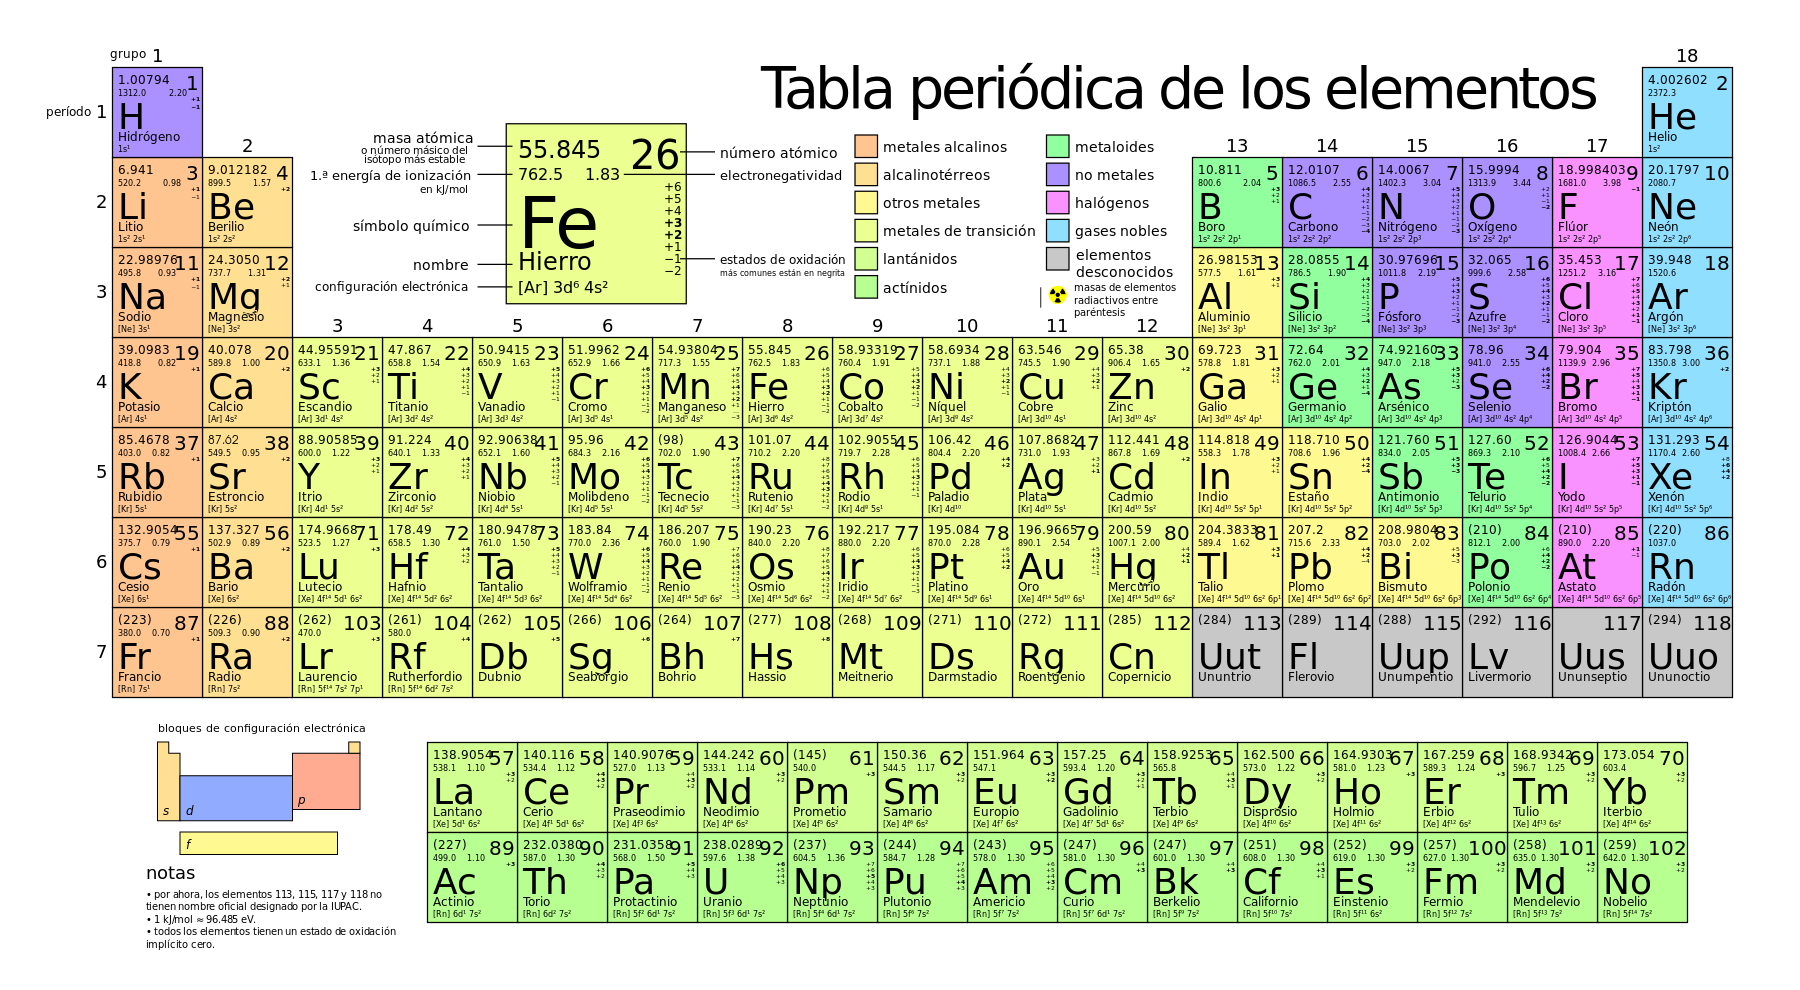
\includegraphics[scale=0.28]{./periodica.png}
%\end{figure}
\section{DOCUMETOS A ENTREGAR}
\begin{itemize}
\item Los ficheros fuentes \emph{ElementoQuimico.java} y \emph{ElementoQuimico.java}
\item El directorio \emph{doc} 
\item Todo los ficheros se comprimen en un único fichero denominado nombreApellidos.tar.gz o nombreApellidos.zip y se sube a la plataforma.  
\end{itemize}
\end{document}